\section{A motivating example: maximum across two vector ISAs}
\label{sec:example}

\todo{Candidate example. The discrepancy and diagnostic measurements below have archived evidence. A complete proof of the repaired final optimized kernel is pending. This example does not establish a speedup over XNNPACK and therefore does not yet satisfy the intended performance narrative.}

Consider an elementwise maximum kernel that reads two binary32 arrays and writes one result per element. Figure~\ref{fig:kernels} shows excerpts from a NEON reference and the final RVV implementation in SALTyRN's published optimized-kernel repository~\cite{final-kernels}. The NEON loop processes four elements at a time. Its tail loads another four elements but stores only the requested prefix. The RVV implementation uses the maximum active length for full blocks and selects a shorter length for the final remainder. These control flows require different arguments about the processed prefix and valid memory accesses. In particular, the NEON tail requires readable padding even when only one output element is requested.

\begin{figure}[t]
\begin{minipage}{\linewidth}
\textbf{NEON: fixed-width main loop}
\lstinputlisting{code/neon-loop.c}
\medskip
\textbf{RVV: full blocks and a variable-length tail}
\lstinputlisting{code/rvv-loop.c}
\end{minipage}
\caption{Excerpts from the unchanged source implementations. Signatures, assertions, and the NEON tail are omitted here; the complete source files are retained in the draft package. The RVV comments are omitted without changing executable statements. \texttt{batch} counts bytes, and \texttt{n} counts float elements. The proof must cover the complete functions, including the omitted tail.}
\label{fig:kernels}
\end{figure}

The numerical operations also differ. For the Arm floating-point profile used in this example, \texttt{vmaxq\_f32} propagates a NaN operand. RVV's \texttt{vfmax} returns the numerical operand when exactly one operand is NaN~\cite{acle,rvv}. Treating both instructions as a single mathematical maximum would erase the difference before any program proof began. The semantic shims instead retain separate lane functions. Figure~\ref{fig:semantics} extracts these functions from the existing QCP shim: the Arm branch quiets signaling NaNs and preserves a NaN result, whereas the RVV branch selects the numerical operand or a canonical NaN. Vector shims apply the appropriate function to the active lanes. This code illustrates existing semantic definitions, not a newly completed hardware-refinement proof.

\begin{figure}[t]
\lstinputlisting{code/max-semantics.c}
\caption{Existing C lane interpretations, with their QCP annotations omitted for space. The helpers inspect binary32 bit patterns and compare non-NaN values. Decimal constants \texttt{4194304U} and \texttt{2143289344U} encode the quiet-NaN bit and a canonical quiet NaN. The original definitions and contracts accompany the excerpts. The modeled Arm profile disables flush-to-zero and default-NaN behavior; floating-point exception flags are outside the output observation.}
\label{fig:semantics}
\end{figure}

The disagreement has a one-element witness:
\[
 n=1,\qquad A[0]=\mathtt{0x7fc12345}\;\text{(quiet NaN)},\qquad
 B[0]=\mathtt{0x3f800000}\;(1.0).
\]
With sufficient input padding and disjoint buffers, executing the compiled kernels under AArch64 and RVV instruction emulation produces NaN and $1.0$, respectively. The RVV result is the same at the three tested hardware vector lengths, 128, 256, and 512 bits. This is a concrete execution discrepancy. It is not a difference in NaN payload or the sign of zero, both of which the output relation in Section~\ref{sec:guarantee} permits.

A diagnostic run of the local SALTyRN bounded checker accepted the same final RVV candidate at input length one and VLEN 512. Inspection showed that its NEON maximum model used the same floating-point maximum operation as the RVV model. In an isolated copy, adding the NEON NaN-propagation case changed the result to a counterexample without changing the kernel pair, input length, or comparison relation. Thus this particular missed discrepancy concerns the semantic model, not the input-length bound. The run used a locally adapted checker and is not a reconstruction of the exact verification run reported in SALTyRN's paper. It also does not demonstrate that QCP automatically synthesizes counterexamples.

To preserve the NEON output behavior, the candidate repair retains the RVV maximum and selects a canonical NaN wherever either operand is NaN:
\begin{lstlisting}
vbool4_t a_nan = __riscv_vmfne_vv_f32m8_b4(va, va, vl);
vbool4_t b_nan = __riscv_vmfne_vv_f32m8_b4(vb, vb, vl);
vbool4_t any_nan = __riscv_vmor_mm_b4(a_nan, b_nan, vl);
vacc = __riscv_vfmerge_vfm_f32m8(
    vacc, __builtin_nanf(""), any_nan, vl);
\end{lstlisting}
The repair is inserted after maximum in both the full-block and tail paths, using \texttt{vlmax} in the former. It leaves the NEON implementation, RVV loop organization, and register grouping unchanged. Regression executions agree under the intended output relation, including mixed exceptional and finite values. \todo{Complete the final optimized kernel's shim bindings, loop and memory obligations, and all dependent proof checks for the same profile as the performance experiment. Historical proofs of an intermediate RVV implementation do not discharge these obligations.}

\begin{figure}[t]
\centering
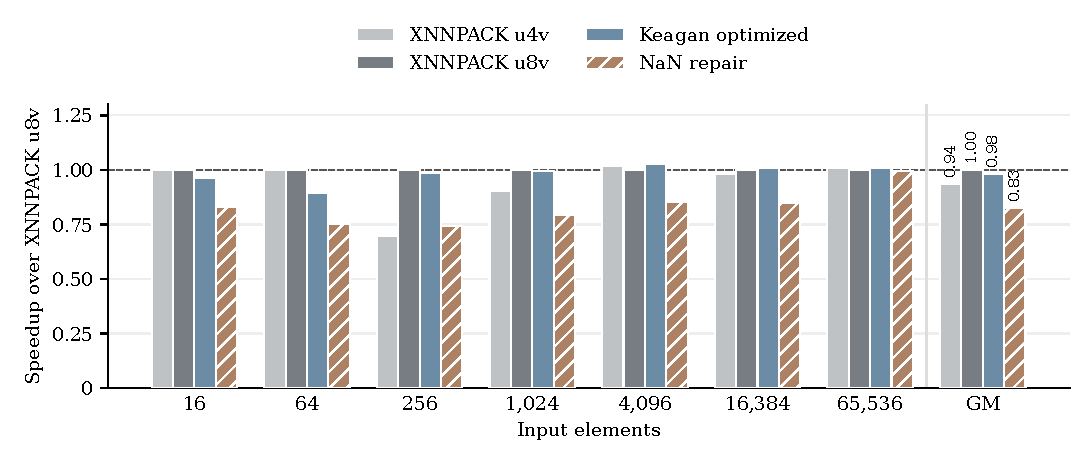
\includegraphics[width=0.96\linewidth]{figures/vmax-performance.pdf}
\caption{Preliminary local Saturn RTL measurements on finite inputs, reproduced from the archived experiment. Speed is XNNPACK RVV u8v cycles divided by the measured implementation's cycles. Each size uses one warm-up and the median of three timed calls within one simulation run; no confidence interval is claimed. Hardware VLEN is 512 bits and datapath width is 256 bits. The published optimized and XNNPACK implementations do not preserve the NEON NaN behavior; the repair adds that behavior. These are measurements, not proof results or a precise reproduction of the SALTyRN paper's configuration.}
\label{fig:vmax-performance}
\end{figure}

The measured geometric-mean speeds relative to XNNPACK u8v are $0.982\times$ for the published optimized candidate and $0.826\times$ for the repair (Figure~\ref{fig:vmax-performance}). The repair increases the geometric mean of the per-size cycle ratios by $18.8\%$. These measurements do not support a claim that this candidate retains a performance advantage over XNNPACK. They instead expose the cost of preserving the selected reference behavior. Whether that behavior is required depends on the contract: XNNPACK's historical min/max discussion explicitly declines a NaN-handling guarantee~\cite{xnn-nan-policy}. Consequently this witness establishes failure of NEON-preserving equivalence, without by itself establishing an XNNPACK API defect.
